% Source printed pp. 175-181 / PDF pp. 183-189.
\section{有限群的商}\label{src:5.2}
\begin{epigraph}
无论你将对称的含义界定得多么宽泛或狭窄, 它始终是人类历代试图理解并创造秩序, 美与完美的一种观念.
\epigraphauthor{Hermann Weyl}
\end{epigraph}
仿射概形对有限抽象群的商叠 $[\Spec A/G]$ 构成一类性质特别好的 Deligne--Mumford 叠. 它们的几何就是 $\Spec A$ 的 $G$-等变几何 (见表~\bookref{1.6.15}). 本节将说明自然映射 $[\Spec A/G]\to\Spec A^G$ 是粗模空间 (定理~\bookref{5.2.3}). 下一节将说明每个 Deligne--Mumford 叠在平展局部都同构于形如 $[\Spec A/G]$ 的商叠 (定理~\bookref{5.3.1}). 结合这两个定理, 将证明粗模空间的存在性, 即 Keel--Mori 定理 (\bookref{5.4.6}).

\subsection{粗模空间与几何商}\label{src:5.2.1-subsection}
\begin{definition}[粗模空间]\label{src:5.2.1}
从代数叠到代数空间的态射 $\pi:\mathcal X\to X$ 称为\newterm{粗模空间}{coarse moduli space}, 若
\begin{enumerate}[(1)]
\item 对每个代数闭域 $k$, 所诱导的映射 $\mathcal X(k)/{\sim}\to X(k)$ 是双射, 其中源是 $\mathcal X$ 在 $k$ 上对象的同构类集合, 且
\item $\pi$ 对到代数空间的映射具有泛性质, 即到代数空间的每个映射 $\mathcal X\to Y$ 都唯一分解为
\[
\begin{tikzcd}
\mathcal X\arrow[d,"\pi"']\arrow[dr]&\\
X\arrow[r,dashed]&Y.
\end{tikzcd}
\]
\end{enumerate}
\end{definition}
\begin{definition}[几何商]\label{src:5.2.2}
若 $G$ 是概形 $S$ 上的 fppf 群概形 (例如对应于有限抽象群的有限群概形), 作用于 $S$ 上的代数空间 $U$, 则 $S$ 上到代数空间的 $G$-不变态射 $U\to X$ 称为\newterm{几何商}{geometric quotient}, 若 $[U/G]\to X$ 是粗模空间, 即
\begin{enumerate}[(1)]
\item 对每个代数闭域 $k$, 映射 $U\to X$ 诱导双射 $U(k)/G\xrightarrow{\sim}X(k)$, 且
\item $U\to X$ 对到代数空间的 $G$-不变映射具有泛性质, 即对到代数空间的每个 $G$-不变映射 $U\to Y$, 存在唯一映射 $X\to Y$, 使得 $U\to Y$ 分解为 $U\to X\to Y$.
\end{enumerate}
\end{definition}
若 $\pi:U\to X$ 是几何商, 常写作 $X=U/G$. 几何商 $U\to U/G$ 分解为
\[
\begin{tikzcd}
U\arrow[r]\arrow[dr,"\text{几何商}"']&{[U/G]}\arrow[d,"\text{粗模空间}"]\\
&U/G.
\end{tikzcd}
\]
当 $G$ 在 $U$ 上自由作用 (即作用映射 $G\times U\to U\times U$ 是单态射) 时, 已定义代数空间商 $U/G$ (推论~\bookref{4.1.14}), 它与几何商等同 (推论~\bookref{5.2.13}).

若有限抽象群 $G$ 作用于仿射概形 $\Spec A$, 则 $G$ 也作用于环 $A$. 定义\newterm{不变量环}{invariant ring} 为
\[
A^G=\{f\in A\mid g\cdot f=f\text{ 对所有 }g\in G\}.
\]
本节的主要结果是 $\Spec A\to\Spec A^G$ 为几何商.
\begin{theorem}\label{src:5.2.3}
若 $G$ 是作用于仿射概形 $\Spec A$ 的有限抽象群, 则 $\pi:[\Spec A/G]\to\Spec A^G$ 是粗模空间. 此外,
\begin{enumerate}[(1)]
\item $\pi$ 是万有同胚;
\item 沿代数空间的平坦态射 $X'\to\Spec A^G$ 对 $\pi$ 作基变换, 得到粗模空间;
\item 自然映射 $\mathcal O_X\to\pi_*\mathcal O_{\mathcal X}$ 是同构; 且
\item 若 $A$ 在 Noether 环 $R$ 上有限生成, 则 $A^G$ 在 $R$ 上有限生成, 且 $\pi$ 固有.
\end{enumerate}
\end{theorem}
概形对有限群的商在许多文献中都有论述, 例如~\cite[\S V.9]{Bou89}, \cite[\S III.12]{Ser88} 和~\cite[第 $66$ 页]{Mum70a}. 下面的证明沿用商概形 $U/G$ 存在性的标准论证, 但要证明它在代数空间范畴中具有泛性质, 还需额外的工作.
\newpage
\begin{example}\label{src:5.2.4}
假设 $\operatorname{char}(k)\neq2$. 若 $G=\mathbb Z/2$ 通过 $-1\cdot x=-x$ 作用于 $\mathbb A^1=\Spec k[x]$, 则 $k[x]^G=k[x^2]$. 几何商是将 $t$ 送到 $t^2$ 的映射 $\mathbb A^1=\Spec k[x]\to\Spec k[x^2]=\mathbb A^1$. 映射 $[\mathbb A^1/G]\to\Spec k[x^2]$ 是粗模空间.

类似地, 若 $G=\mathbb Z/2$ 通过 $-1\cdot(x,y)=(-x,-y)$ 作用于 $\mathbb A^2=\Spec k[x,y]$, 则 $k[x,y]^G=k[x^2,xy,y^2]$, 几何商为 $\mathbb A^2\to\mathbb A^2/G=\Spec k[x^2,xy,y^2]$. 置 $A=x^2$, $B=xy$, $C=y^2$, 不变量环可与 $k[A,B,C]/(B^2-AC)$ 等同, 因此商 $\mathbb A^2/G$ 是二次曲线上的锥, 特别地它有奇点.
\begin{figure}[H]
\centering\refstepcounter{figure}\label{src:5.2.5}
% Source PDF p. 185, artwork retained at 400 DPI.
\begin{tikzpicture}
\node[anchor=south west,inner sep=0] (art) at (0,0)
  {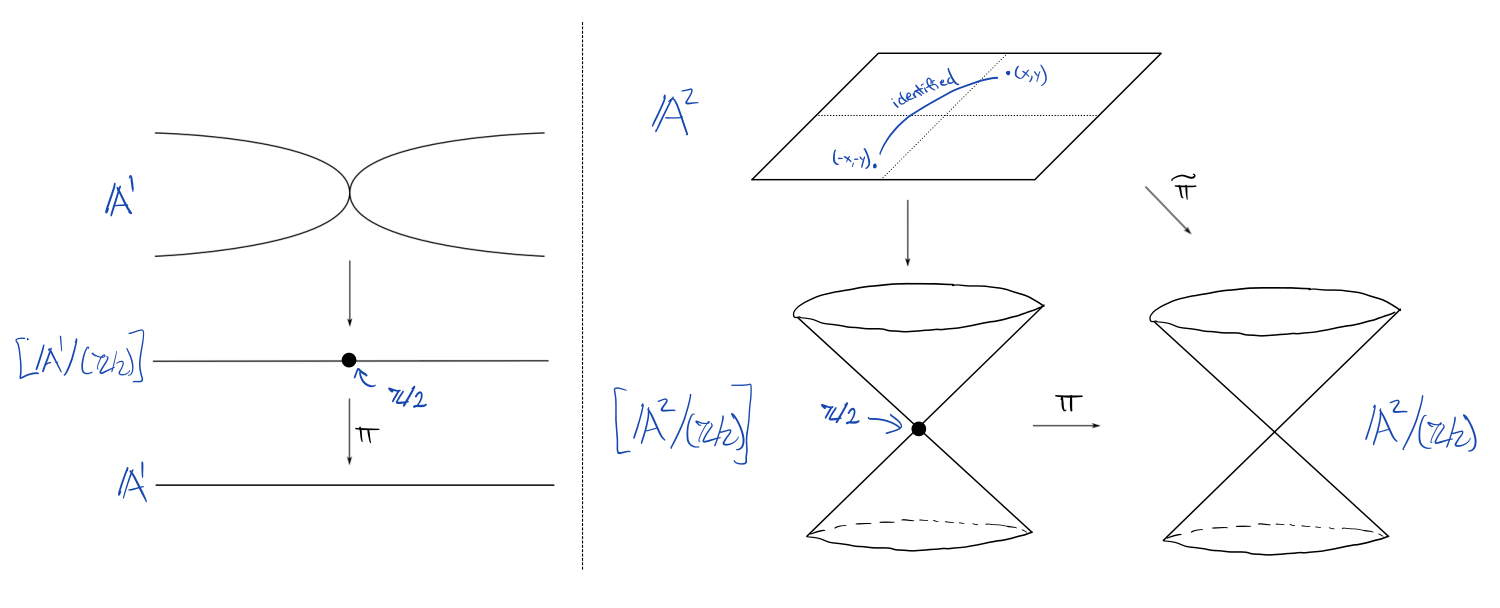
\includegraphics[width=0.95\textwidth]{figures/finite-quotients-source.png}};
\begin{scope}[x={(art.south east)},y={(art.north west)}]
\node[rotate=27,fill=white,inner sep=0.4pt,minimum width=2.7em,font=\scriptsize,text=blue!65!black]
 at (0.618,0.858) {等同};
\end{scope}
\end{tikzpicture}

\end{figure}
\end{example}

\subsection{不变量环的性质}\label{src:5.2.2-subsection}
\begin{lemma}\label{src:5.2.6}
若有限抽象群 $G$ 通过 $R$-代数自同构作用于 $R$-代数 $A$, 则 $A^G\to A$ 整. 若 $R$ 是 Noether 环且 $A$ 在 $R$ 上有限生成, 则 $A^G\to A$ 有限, 且 $A^G$ 在 $R$ 上有限生成.
\end{lemma}
\begin{proof}
为说明 $A^G\to A$ 整, 注意对每个元素 $a\in A$, 乘积 $\prod_{g\in G}(x-ga)\in A^G[x]$ 是具有不变系数且以 $a$ 为根的多项式. 若 $R$ 是 Noether 环, $R\to A$ 有限型, 则 $A^G\to A$ 也有限型. 由于 $A^G\to A$ 整且有限型, 它有限 (参见~\cite[推论 $5.2$]{AM69}). 由于 $R$ 是 Noether 环, 由 Artin--Tate 引理 (参见~\cite[命题 $7.8$]{AM69}) 可得 $R\to A^G$ 有限型.
\end{proof}
不变量环与平坦基变换相容.
\begin{lemma}\label{src:5.2.7}
设 $G$ 是作用于仿射概形 $\Spec A$ 的有限抽象群. 若 $A^G\to B$ 是平坦环同态, 则 $G$ 作用于仿射概形 $\Spec(B\otimes_{A^G}A)$, 且 $B=(B\otimes_{A^G}A)^G$.
\end{lemma}
\begin{proof}
按定义, 不变量环是等化子
\[
\begin{tikzcd}[column sep=large]
0\arrow[r]&A^G\arrow[r]&A\arrow[r,shift left,"p_1"]\arrow[r,shift right,"p_2"']&\displaystyle\prod_{g\in G}A,
\end{tikzcd}
\]
其中 $p_1(f)=(f)_{g\in G}$, $p_2(f)=(gf)_{g\in G}$. 由于 $A^G\to B$ 平坦,
\[
\begin{tikzcd}[column sep=large]
0\arrow[r]&B\arrow[r]&A\otimes_{A^G}B\arrow[r,shift left,"p_1"]\arrow[r,shift right,"p_2"']&\displaystyle\prod_{g\in G}A\otimes_{A^G}B
\end{tikzcd}
\]
也正合, 因而 $B=(B\otimes_{A^G}A)^G$.
\end{proof}
\newpage
\begin{exercise}\label{src:5.2.8}
设 $A^G\to B$ 是环同态, 考虑交换图
\[
\begin{tikzcd}[column sep=1.7em]
&\Spec B\otimes_{A^G}A\arrow[r]\arrow[d]\arrow[dl]&\Spec A\arrow[d]\\
\Spec(B\otimes_{A^G}A)^G\arrow[r]&\Spec B\arrow[r]\arrow[ur,phantom,"\square" description]&\Spec A^G.
\end{tikzcd}
\]
\begin{enumerate}[(a)]
\item 证明 $\Spec(B\otimes_{A^G}A)^G\to\Spec B$ 是整同胚.
\item 若 $|G|$ 在 $A$ 中可逆, 证明 $B\to(B\otimes_{A^G}A)^G$ 是同构.
\item 给出 $B\to(B\otimes_{A^G}A)^G$ 不是同构的例子.

\textit{提示:} 在特征 $p$ 时, 考虑 $\mathbb Z/p$ 在 $A=k[x,y]$ 上的作用, 其中生成元作用为 $(x,y)\mapsto(x+y,y)$, 并取 $B=A^G/(y)$.
\end{enumerate}
\end{exercise}

\subsection{粗模空间的性质}\label{src:5.2.3-subsection}
\begin{lemma}\label{src:5.2.9}
设 $\pi:\mathcal X\to X$ 是粗模空间, 满足对来自仿射概形的每个平展态射 $X'\to X$, 基变换 $\mathcal X\times_X X'\to X'$ 都是粗模空间. 则自然映射 $\mathcal O_X\to\pi_*\mathcal O_{\mathcal X}$ 是同构.
\end{lemma}
\begin{proof}
由于 $\pi$ 对到代数空间的映射具有泛性质, $\operatorname{Map}(X,\mathbb A^1)\to\operatorname{Map}(\mathcal X,\mathbb A^1)$ 是双射, 换言之, $\Gamma(X,\mathcal O_X)\cong\Gamma(\mathcal X,\mathcal O_{\mathcal X})$. 对每个平展映射 $X'\to X$, 基变换 $\mathcal X'=\mathcal X\times_X X'\to X'$ 也是粗模空间, 故 $\Gamma(X',\mathcal O_{X'})\cong\Gamma(\mathcal X',\mathcal O_{\mathcal X'})$. 这说明 $\mathcal O_X\to\pi_*\mathcal O_{\mathcal X}$ 是同构.
\end{proof}
为粗模空间的性质是平展局部的.
\begin{lemma}\label{src:5.2.10}
设 $\pi:\mathcal X\to X$ 是到代数空间的态射. 假设存在平展覆盖 $\{X_i\to X\}$, 使得对每个 $i$, $\mathcal X\times_X X_i\to X_i$ 是粗模空间. 则 $\pi:\mathcal X\to X$ 是粗模空间.
\end{lemma}
\begin{proof}
粗模空间的公理 (1) 是关于几何纤维的条件, 因而可在平展局部检验, 而公理 (2) 由代数空间是平展拓扑中的层这一事实推出.
\end{proof}

\subsection{\texorpdfstring{$\Spec A\to\Spec A^G$}{Spec A → Spec AG} 是几何商}\label{src:5.2.4-subsection}
\begin{proposition}\label{src:5.2.11}
若 $G$ 是作用于仿射概形 $\Spec A$ 的有限抽象群, 则 $\Spec A\to\Spec A^G$ 是几何商.
\end{proposition}
\begin{proof}
考虑交换图
\[
\begin{tikzcd}
U=\Spec A\arrow[d]\arrow[dr,"\widetilde\pi"]&\\
\mathcal X={[U/G]}\arrow[r,"\pi"']&X=\Spec A^G.
\end{tikzcd}
\]
由于 $\widetilde\pi$ 整且支配, 它满射. 为说明 $\widetilde\pi$ 在几何点的 $G$-轨道上单射, 设 $k$ 是代数闭域, 假设 $x,x'\in U(k)$ 在 $U\times_X k$ 上诱导的 $G$-作用下具有不同的 $G$-轨道. 由于这些轨道不交, 存在函数 $f\in A\otimes_{A^G}k$, 满足 $f|_{Gx}=0$, $f|_{Gx'}=1$. 则 $\widetilde f=\prod_{g\in G}gf\in(A\otimes_{A^G}k)^G$ 是 $G$-不变函数, 满足 $\widetilde f(x)=0$, $\widetilde f(x')=1$, 这蕴含 $\widetilde\pi(x)\neq\widetilde\pi(x')\in X(k)$.

还需说明自然映射
\begin{equation}\label{src:5.2.12}
\operatorname{Map}(X,Y)\longrightarrow\operatorname{Map}(\mathcal X,Y)
\end{equation}
对每个代数空间 $Y$ 都是双射. 注意当 $Y$ 仿射时这显然成立, 因为 $\Gamma(\mathcal X,\mathcal O_{\mathcal X})=\Gamma(X,\mathcal O_X)$. (当 $Y$ 是概形时, 不难归结到此情形: 若 $g:\mathcal X\to Y$ 是映射, 则 $Y$ 的仿射覆盖 $Y_i$ 诱导 $X$ 的开覆盖 $X_i=X\setminus\pi(\mathcal X\setminus g^{-1}(Y_i))$, $g$ 限制为映射 $\pi^{-1}(X_i)\to Y_i$, 由于 $\pi_*\mathcal O_{\mathcal X}=\mathcal O_X$, 它唯一经过 $X_i$ 分解; 另见~\cite[\S$0.6$]{GIT}.)

对于~\bookeqref{5.2.12} 的单射性, 设 $h_1,h_2:X\to Y$ 是满足 $h_1\circ\pi=h_2\circ\pi$ 的两个映射. 设 $E\to X$ 是 $h_1,h_2$ 的等化子, 即沿 $(h_1,h_2):X\to Y\times Y$ 拉回对角线 $Y\to Y\times Y$ 所得. 等化子 $E\to X$ 是单态射且局部有限型. 按构造 $\pi:\mathcal X\to X$ 经过 $E\to X$ 分解, 且由于 $\pi$ 普遍闭且\newterm{概形性支配}{schematically dominant} (即 $\mathcal O_X\to\pi_*\mathcal O_{\mathcal X}$ 单射), $E\to X$ 也如此. 每个普遍闭且局部有限型的单态射都是闭浸入 (见注记~\bookref{A.7.6}), 故 $E\to X$ 是同构.

对于~\bookeqref{5.2.12} 的满射性, 设 $g:\mathcal X\to Y$ 是态射. 先作一些容易的归约. 由引理~\bookref{5.2.7} 和~\bookref{5.2.10}, 问题在 $X$ 上是平展局部的; 特别地, 可假设 $X$ 仿射. 此外, 由于 $\mathcal X$ 拟紧, 映射 $g:\mathcal X\to Y$ 经过 $Y$ 的一个拟紧开代数子空间分解, 故可假设 $Y$ 拟紧. 设 $Y'\to Y$ 是来自仿射概形的平展呈示, 置 $\mathcal X':=\mathcal X\times_Y Y'$.

我们断言, 将 $X$ 换成平展覆盖 $V\to X$, 并将 $\mathcal X$ 换成基变换 $\mathcal X\times_X V$ 后, 在交换图
\[
\begin{tikzcd}
\mathcal X'\arrow[r]\arrow[d,"{g'}"']&\mathcal X\arrow[l,bend right=35,"s"']\arrow[r,"\pi"]\arrow[d,"g"]&X\arrow[dl,dashed]\\
Y'\arrow[r]\arrow[ur,phantom,"\square" description]&Y&
\end{tikzcd}
\]
中存在 $\mathcal X'\to\mathcal X$ 的截面 $s:\mathcal X\to\mathcal X'$.

\bookeqref{5.2.12} 的满射性由此断言推出: 由于 $X$ 与 $Y'$ 仿射, 等式 $\Gamma(X,\mathcal O_X)=\Gamma(\mathcal X,\mathcal O_{\mathcal X})$ 蕴含 $\mathcal X\xrightarrow{s}\mathcal X'\xrightarrow{g'}Y'$ 经由一个态射 $X\to Y'$ 通过 $\pi:\mathcal X\to X$ 分解. 复合 $X\to Y'\to Y$ 给出上图所需的虚线箭头.

为证明此断言, 使用极限方法进一步归结到 $X=\Spec A^G$ 为严格 Hensel 局部环的谱的情形. 对 $U:=\Spec A$ 中位于 $x\in|\mathcal X|$ 上方的闭点 $u$, 严格 Hensel 化 $X^{\mathrm{sh}}:=\mathcal O^{\mathrm{sh}}_{X,\pi(x)}$ 是所有 $\pi(x)$ 的仿射平展邻域 $X_\lambda\to X$ 的极限 $\lim_\lambda X_\lambda$. 基变换 $U^{\mathrm{sh}}:=U\times_X X^{\mathrm{sh}}$ 是仿射概形 $U_\lambda:=U\times_X X_\lambda$ 的极限. 再置 $\mathcal X^{\mathrm{sh}}:=\mathcal X\times_X X^{\mathrm{sh}}=[U^{\mathrm{sh}}/G]$, $\mathcal X_\lambda:=\mathcal X\times_X X_\lambda=[U_\lambda/G]$. 由于 $\mathcal X'\to\mathcal X$ 局部有限表现, 自然映射
\[
\mathrm{colim}_\lambda\operatorname{Mor}_{\mathcal X}(\mathcal X_\lambda,\mathcal X')\longrightarrow\operatorname{Mor}_{\mathcal X}(\mathcal X^{\mathrm{sh}},\mathcal X')
\]
是等价; 这由习题~\bookref{4.3.33} 推出 (该习题断言当第一项 $\mathcal X_\lambda$ 与 $\mathcal X^{\mathrm{sh}}$ 仿射时有此等式), 只需将 $\operatorname{Mor}_{\mathcal X}(\mathcal X^{\mathrm{sh}},\mathcal X')$ 表为 $\operatorname{Mor}_{\mathcal X}(U^{\mathrm{sh}},\mathcal X')\rightrightarrows\operatorname{Mor}_{\mathcal X}(G\times U^{\mathrm{sh}},\mathcal X')$ 的等化子, 左侧也同样处理. $\mathcal X'\times_{\mathcal X}\mathcal X^{\mathrm{sh}}\to\mathcal X^{\mathrm{sh}}$ 的截面由 $\mathcal X$ 上的映射 $\mathcal X^{\mathrm{sh}}\to\mathcal X'$ 确定. 该映射对某个 $\lambda$ 延伸为态射 $\mathcal X_\lambda\to\mathcal X'$, 给出所需截面.

设 $\kappa$ 是 $A^G$ 的剩余域. 由于 $A^G\to A$ 有限, $A=A_1\times\cdots\times A_r$ 是严格 Hensel 局部环的乘积, 每个因子都在 $A^G$ 上有限 (命题~\bookref{B.5.10}). 若 $u\in\Spec A_1\subseteq\Spec A$ 是闭点, 则 $\Spec A_1$ 是 $G_u$-不变的, 轨道 $Gu$ 与 $\Spec A$ 的 $r$ 个连通分支一一对应. 有同构 $\mathcal X\cong[\Spec A_1/G_u]$; 这可直接验证, 例如用 $\Spec A_1\hookrightarrow\Spec A$ 对群胚 $G\times\Spec A\rightrightarrows\Spec A$ 作切片 (如习题~\bookref{4.4.20}). 因此可将 $\mathcal X=[\Spec A/G]$ 换成 $[\Spec A_1/G_u]$, 并假设存在唯一闭点 $u\in\Spec A$, 且 $G$ 在集合意义下固定它. 由于 $Y'\to Y$ 可由概形表出, 可对某个概形 $U'$ 写成 $\mathcal X'=[U'/G]$. 设 $u'\in U'$ 是 $u\in\Spec A$ 的一个原像. 由于 $A$ 严格 Hensel, 且 $G$-等变态射 $U'\to U$ 是平展态射 $Y'\to Y$ 的基变换, 有 $\kappa(u')=\kappa(u)$, $G_{u'}=G_u=G$, 此外稳定子在剩余域上的作用平凡. 再次利用 $A$ 严格 Hensel, 存在唯一截面 $s:\Spec A\to U'$, 满足 $s(u)=u'$ (命题~\bookref{B.5.9}). 此截面 $G$-不变, 因为对每个 $g\in G$, $s\circ g$ 与 $g\circ s$ 都是 $U'\to\Spec A\xrightarrow{g^{-1}}\Spec A$ 的截面, 满足 $u'\mapsto u$, 故由截面的唯一性有 $s\circ g=g\circ s$. 于是 $s:\Spec AS\to U$ 下降为 $\mathcal X'\to\mathcal X$ 的截面 $\mathcal X=[\Spec A/G]\to[U'/G]=\mathcal X'$. 至此证明了 $\Spec A\to\Spec A^G$ 是几何商.
\end{proof}
现在不仅可得 $[\Spec A/G]\to\Spec A^G$ 是粗模空间, 还可得它具有定理~\bookref{5.2.3} 的性质 (1)--(4).
\begin{proof}[定理~\bookref{5.2.3} 的证明]
命题~\bookref{5.2.11} 蕴含 $\pi:[\Spec A/G]\to\Spec A^G$ 是粗模空间. 为说明性质 (1), 即 $\pi$ 是万有同胚, 注意由于 $\pi$ 双射且闭, 其集合意义下的逆映射连续, 故 $\pi$ 是同胚. 沿态射 $\Spec B\to\Spec A^G$ 对 $\pi$ 作基变换, 分解为
\[
{[\Spec(B\otimes_{A^G}A)/G]}\longrightarrow\Spec(B\otimes_{A^G}A)^G\longrightarrow\Spec B,
\]
其中第一映射由上述论证为同胚, 第二映射由习题~\bookref{5.2.8} 为同胚. 性质 (2), 即沿平坦态射 $X'\to\Spec A^G$ 对 $\pi$ 作基变换仍是粗模空间, 可先用引理~\bookref{5.2.10} 归结到 $X'$ 仿射的情形, 再由引理~\bookref{5.2.7} 推出. 性质 (3), 即 $\mathcal O_X\to\pi_*\mathcal O_{\mathcal X}$ 为同构, 由 (2) 及引理~\bookref{5.2.9} 直接推出. 最后, 引理~\bookref{5.2.6} 蕴含 (4): 若 $R$ 是 Noether 环, $R\to A$ 有限型, 则 $R\to A^G$ 有限型. 特别地, $A^G\to A$ 有限型, 而 $\pi:[\Spec A/G]\to\Spec A^G$ 分离, 普遍闭且有限型, 即固有.
\end{proof}
\begin{corollary}\label{src:5.2.13}
设 $G$ 是在仿射概形 $U=\Spec A$ 上自由作用的有限抽象群, 则代数空间商 $U/G$ 同构于 $\Spec A^G$.
\end{corollary}
\begin{proof}
代数空间商与几何商都对到代数空间的映射具有泛性质.
\end{proof}
\begin{exercise}\label{src:5.2.14}
设 $G$ 是作用于概形 $U$ 的有限抽象群.
\begin{enumerate}[(a)]
\item 证明几何商 $U/G$ 是概形, 当且仅当每个 $G$-轨道都包含在一个仿射开子概形中.
\item 若 $U$ 是 Noether 环 $R$ 上的仿射 (分别为拟仿射, 拟射影, 射影) 概形, 证明 $U/G$ 是 $R$ 上的仿射 (分别为拟仿射, 拟射影, 射影) 概形.
\end{enumerate}
\end{exercise}
\begin{exercise}\label{src:5.2.15}
假设有限抽象群 $G$ 作用于 Noether 环 $R$ 上的有限型仿射概形 $\Spec A$. 若 $x\in\Spec A$ 是闭点, 证明 $\Spec A$ 在 $x$ 处的完备化的 $G_x$-不变量与 $\Spec A^G$ 在 $x$ 的像处的完备化之间有同构
\[
\widehat A^{G_x}\cong\widehat{A^G}.
\]
\end{exercise}
以下习题将定理~\bookref{5.2.3} 从有限群的商推广到有限平坦群胚的商.
\begin{exercise}[困难]\label{src:5.2.16}
设 $s,t:R\rightrightarrows U$ 是仿射概形的有限平坦群胚, 定义 $A^R\subseteq A$ 为 $R$-不变量子环, 即由满足 $s^*a=t^*a\in\Gamma(R,\mathcal O_R)$ 的元素 $a\in A$ 组成的子环. 证明 $[U/R]\to X:=\Spec A^R$ 是具有定理~\bookref{4.4.13} 中性质 (1)--(4) 的粗模空间.

\textit{提示:} 为说明 $A^R\to A$ 整, 对元素 $a\in A$, 不使用引理~\bookref{5.2.6} 证明中的乘积 $\prod_{g\in G}(x-ga)\in A^G[x]$, 而使用 $\delta_0(a)\in B$ 的特征多项式, 其中将 $B$ 经由 $\delta_1$ 视作 $A$ 上的局部自由模, $\delta_0,\delta_1:A\rightrightarrows B=\Gamma(U,\mathcal O_U)$ 是两个有限平坦环映射. 另见~\cite[定理 V.4.1]{SGA3I}, \cite[命题 $5.1$]{KM97}, \cite[定理 $3.1$]{Con05b}, \cite[定理 $6.2.2$]{Ols16} 和~\cite[Tag 0DUR]{SP}.
\end{exercise}
